\newif\ifglobal

%%%%%%%%%%%%%%%%%%%%%%%
%%% Compile to view %%%
%%%%%%%%%%%%%%%%%%%%%%%

%%%%%%%%%%%%%%%%%%%%%%%%%%%%%%%%%%%%%%%%%%%%%%%%%%%
%%% Readme:                                     %%%
%%% https://www.overleaf.com/read/bwdjvfjksvjy/ %%%
%%%%%%%%%%%%%%%%%%%%%%%%%%%%%%%%%%%%%%%%%%%%%%%%%%%

% >>> M?: marks a module setting number or important notice

% >>> M4: Set {./relative-path} to external files for this module <<<
\def \modulefiles {./31-SENSOR}
% To add an external file, use:
% (Replace '---' with actual filename)
% '\input{\modulefiles/tables/---.tex}' for tables
% '\includegraphics{\modulefiles/figures/---}' for figures
% '\subfile{\modulefiles/---}' for register files

% >>> M1: This module is in global project? <<<
% 'YES' - uncomment; 'NO' - comment out
\globaltrue

\ifglobal
    \documentclass[main\_\_EN.tex]{subfiles}

\else
    \documentclass[openany, 10pt]{book}

    % >>> M2: In ./00-shared/preamble-trm-module, also find
    %         settings for visibility of todo notes, watermark <<<
    \usepackage{preamble-trm-module}

    % >>> M3: Temporary labels in English,
    %         you can add your own labels there <<<
    \myexternaldocument{./00-shared/temp-labels-en}

\fi %\ifglobal


\setcounter{secnumdepth}{4}


% >>> M5: If this module needs any updates in
% './00-shared/preamble-trm-module.sty'
% (include additional package, etc.), contact your module PM
% or create the file './00-shared/changelog.tex' make the
% necessary updates yourself and document them in this file <<<

% Make text left-aligned and allow latex to break pages naturally, comment out for full justification
\raggedright
\raggedbottom


\begin{document}


% Sets language into which pre-defined bits of text are translated
\selectlanguage{english}
\setenglishformatting

% Do not delete this block
\ifglobal
% Add the following front matter if
% this module is outside of global project
\else
    \InputIfFileExists{readme}{}{}
    \listoftodos
    {\let\clearpage\relax \listofdonetodos}
    \tableofcontents
    %\listoftables
    %\listoffigures
\fi


%%%%%%%%%%%%%%%%%%%%%%%%%
%%% TRM Module Begins %%%
%%%%%%%%%%%%%%%%%%%%%%%%%

\hypertarget{sensor}{}
\chapter{On-Chip Sensors and Analog Signal Processing}
\label{mod:sensor}

\section{Introduction}

ESP32 has a \hyperref[ssec:touch sensor]{capacitive touch sensor} with up to 10 inputs. 

The processing of analog signals is done by two \hyperref[ssec:saradc]{successive approximation ADCs} (SAR ADC). There are five controllers dedicated to operating ADCs. This provides flexibility when it comes to converting analog inputs in both high-performance and low-power modes, with minimum processor overhead.

ESP32 is also capable of generating analog signals, using two \hyperref[ssec:dac]{independent DACs} and a \hyperref[ssec:cosine gen]{cosine waveform generator}.

\section{Capacitive Touch Sensor}\label{ssec:touch sensor}

\subsection{Introduction}

A touch-sensor system is built on a substrate which carries electrodes and relevant connections under a protective flat surface; see Figure \ref{figure:touch sensor}. When a user touches the surface, the capacitance variation is triggered and a binary signal is generated to indicate whether the touch is valid.

\begin{figure}[!ht]
    \centering
    \fbox{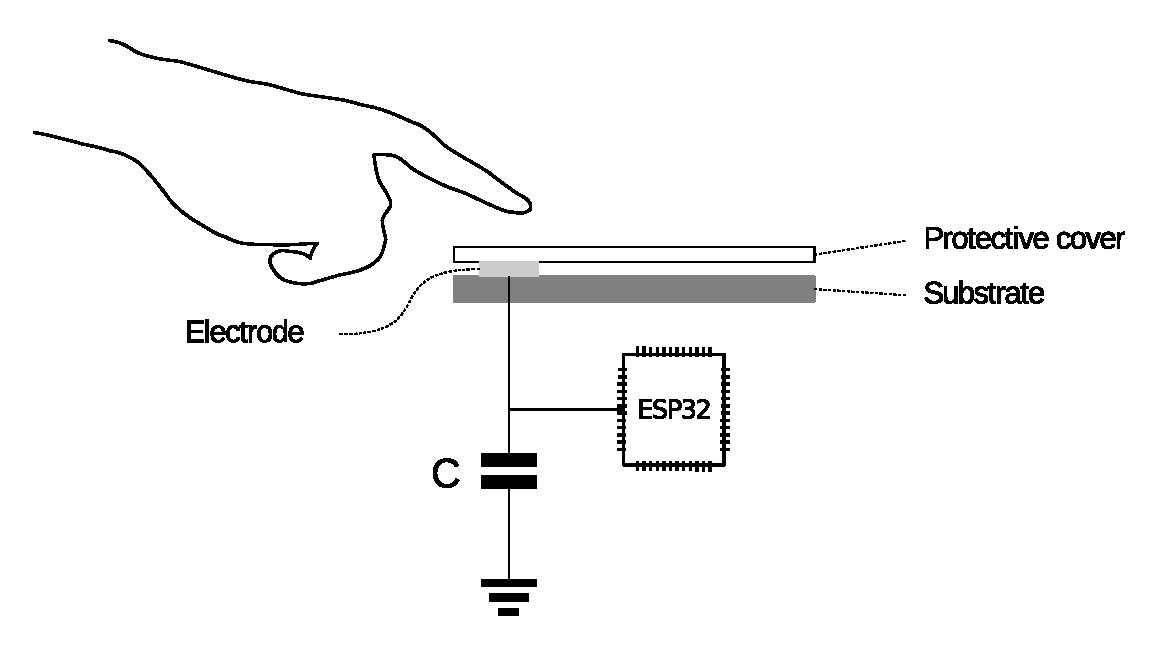
\includegraphics[width=0.6\textwidth]{./31-SENSOR/figures/touchsensor2.eps}}
    \caption{Touch Sensor}
    \label{figure:touch sensor}
\end{figure}

\subsection{Features}\label{sec:on_chip_sensor_features}

\begin{itemize}
    \item Up to 10 capacitive touch pads / GPIOs
    \item The sensing pads can be arranged in different combinations, so that a larger area or more points can be detected.
    \item The touch pad sensing process is under the control of a hardware-implemented finite-state machine (FSM) which is initiated by software or a dedicated hardware timer.
    \item Information that a pad has been touched can be obtained:
    \begin{itemize}
        \item by checking touch-sensor registers directly through software,
        \item from an interrupt triggered by a touch detection,
        \item by waking up the CPU from deep sleep upon touch detection.
    \end{itemize}
    \item Support for low-power operation in the following scenarios:
    \begin{itemize}
        \item CPU waiting in deep sleep and saving power until touch detection and subsequent wake up
        \item Touch detection managed by the ULP coprocessor \\
        The user program in ULP coprocessor can trigger a scanning process by checking and writing into specific registers, in order to verify whether the touch threshold is reached.
    \end{itemize}
\end{itemize}

\begin{tiplisting}
ESP32 Touch Sensor has not passed the Conducted Susceptibility (CS) test for now, and thus has limited application scenarios. 
\end{tiplisting}

\subsection{Available GPIOs}

All 10 available sensing GPIOs (pads) are listed in Table \ref{table:touch pads}.

\begin{longtable}[c]{|p{7.5cm}|p{7.5cm}|}
    \caption{ESP32 Capacitive Sensing Touch Pads}
    \label{table:touch pads}
    \\\hline
    \rowcolor{lightgray}
    Touch Sensing Signal Name & Pin Name \\
    \hline
    \endfirsthead
    \hline
    \rowcolor{lightgray}
    Touch Sensing Signal Name & Pin Name \\
    \hline
    \endhead
    \endfoot
    \endlastfoot
    T0  &  GPIO4 \\\hline
    T1  &  GPIO0 \\\hline
    T2  &  GPIO2 \\\hline
    T3  &  MTDO  \\\hline
    T4  &  MTCK  \\\hline
    T5  &  MTDI  \\\hline
    T6  &  MTMS  \\\hline
    T7  &  GPIO27 \\\hline
    T8  &  32K\_XN \\\hline
    T9  &  32K\_XP \\\hline
\end{longtable}

\subsection{Functional Description}
\label{figure:touch sensor func desc}

The internal structure of the touch sensor is shown in Figure \ref{figure:touch sensor structure}. The operating flow is shown in Figure \ref{figure:touch sensor operating flow}.

\begin{figure}[!ht]
    \centering
    \fbox{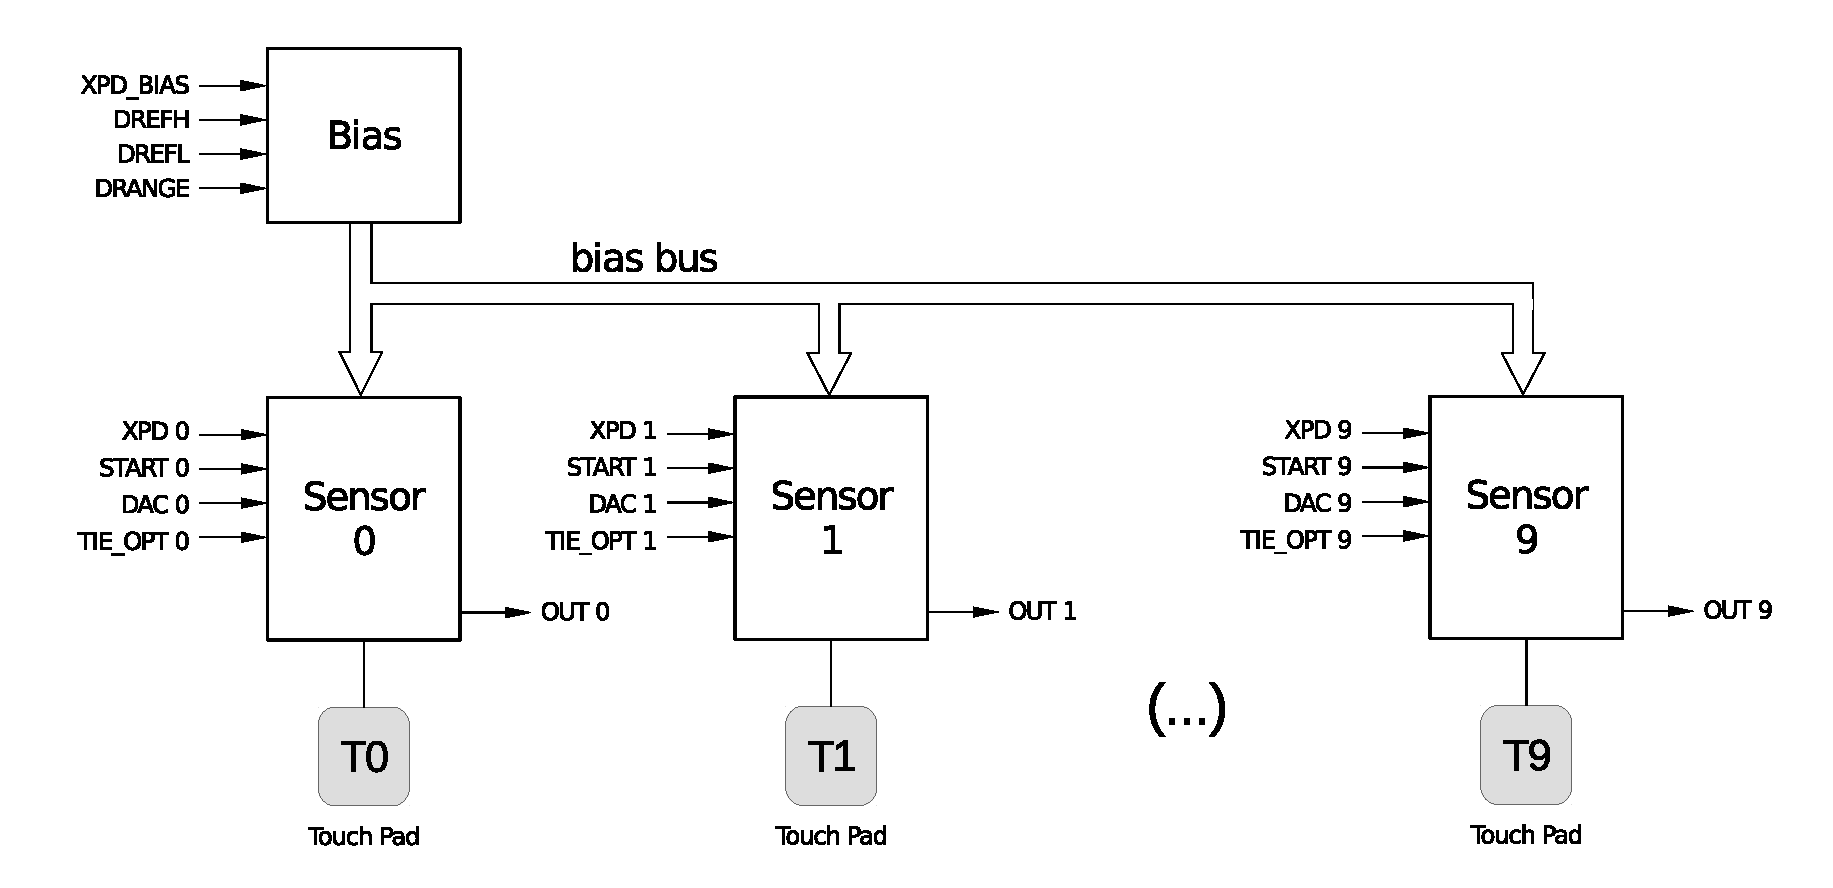
\includegraphics[width=0.7\textwidth]{./31-SENSOR/figures/Touch_Sensor.eps}}
    \caption{Touch Sensor Structure}
    \label{figure:touch sensor structure}
\end{figure}

The capacitance of a touch pad is periodically charged and discharged. The chart "Pad Voltage" shows the charge/discharge voltage that swings from DREFH (reference voltage high) to DREFL (reference voltage low). During each swing, the touch sensor generates an output pulse, shown in the chart as "OUT". The swing slope is different when the pad is touched (high capacitance) and when it is not (low capacitance). By comparing the difference between the output pulse counts during the same time interval, we can conclude whether the touch pad has been touched. \hyperref[regdesc:RTCIOTOUCHPADnREG]{TIE\_OPT} is used to establish the initial voltage level that starts the charge/discharge cycle.

\begin{figure}[!ht]
    \centering
    \fbox{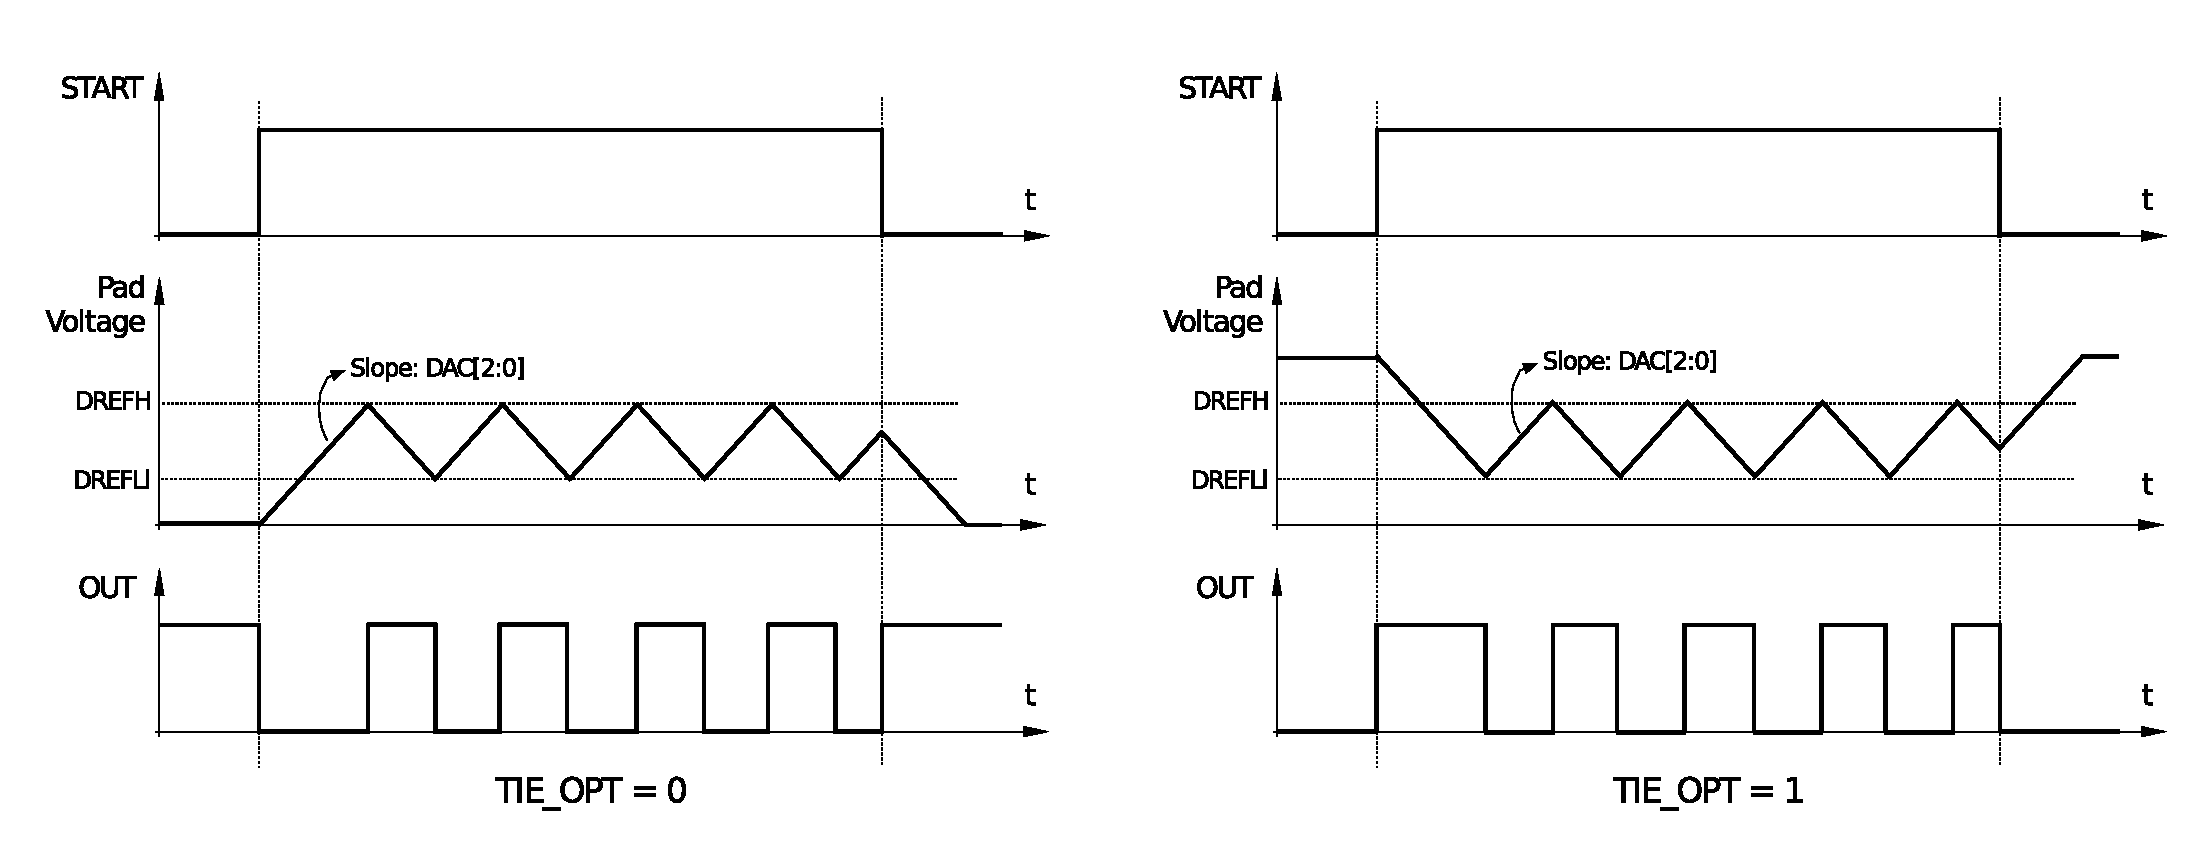
\includegraphics[width=0.9\textwidth]{./31-SENSOR/figures/Touch_Sensor2.eps}}
    \caption{Touch Sensor Operating Flow}
    \label{figure:touch sensor operating flow}
\end{figure}

\subsection{Touch FSM}

The Touch FSM performs a measurement sequence described in section \ref{figure:touch sensor func desc}. Software can operate the Touch FSM through dedicated registers. The internal structure of a touch FSM is shown in Figure \ref{figure:touch fsm}.

The functions of Touch FSM include:
\begin{itemize}
    \item Receipt of a start signal, either from software or a timer
    \begin{itemize}
        \item when \hyperref[regdesc:SENSSARTOUCHCTRL2REG]{SENS\_SAR\_TOUCH\_START\_FORCE}=1, \hyperref[regdesc:SENSSARTOUCHCTRL2REG]{SENS\_SAR\_TOUCH\_START\_EN} is used to initiate a single measurement
        \item when \hyperref[regdesc:SENSSARTOUCHCTRL2REG]{SENS\_SAR\_TOUCH\_START\_FORCE}=0, measurement is triggered periodically with a timer.
    \end{itemize}
    The Touch FSM can be active in sleep mode. The \hyperref[regdesc:SENSSARTOUCHCTRL2REG]{SENS\_SAR\_TOUCH\_SLEEP\_CYCLES} register can be used to set the cycles. The sensor is operated by RTC\_FAST\_CLK, which normally runs at 8 MHz. More information on that can be found in chapter \hyperref[mod:resclk]{Reset and Clock}.
    \item Generation of XPD\_TOUCH\_BIAS / TOUCH\_XPD / TOUCH\_START with adjustable timing sequence \\
    To select enabled pads, TOUCH\_XPD / TOUCH\_START is masked by the 10-bit register \hyperref[regdesc:SENSSARTOUCHENABLEREG]{SENS\_SAR\_TOUCH\\\_PAD\_WORKEN}.
    \item Counting of pulses on TOUCH0\_OUT \verb+~+ TOUCH9\_OUT\\
    The result can be read from \hyperref[regdesc:SENSSARTOUCHOUT1REG]{SENS\_SAR\_TOUCH\_MEAS\_OUT\textcolor{red}{\it{n}}}. All ten touch sensors can work simultaneously.
    \item Generation of a wakeup interrupt\\
    The FSM regards the touch pads as “touched”, if the number of counted pulses is below the threshold. The 10-bit registers \hyperref[regdesc:SENSSARTOUCHENABLEREG]{SENS\_TOUCH\_PAD\_OUTEN1} \& \hyperref[regdesc:SENSSARTOUCHENABLEREG]{SENS\_TOUCH\_PAD\_OUTEN2} define two sets of touch pads, i.e. SET1 \& SET2. If at least one of the pads in SET1 is “touched”, the wakeup interrupt will be generated by default. It is also possible to configure the wakeup interrupt to be generated only when pads from both sets are “touched”.
\end{itemize}

\begin{figure}[!ht]
    \centering
    \fbox{
\includegraphics[width=0.8\textwidth]{./31-SENSOR/figures/touch_fsm.eps}}
    \caption{Touch FSM Structure}
    \label{figure:touch fsm}
\end{figure}

\section{SAR ADC}\label{ssec:saradc}

\subsection{Introduction}

ESP32 integrates two 12-bit SAR ADCs. They are managed by five SAR ADC controllers, and are able to measure signals from one to 18 analog pads.

The SAR ADC controllers have specialized uses. Two of them support high-performance multiple-channel scanning. Another two are used for low-power operation during Deep-sleep, and the last one is dedicated to PWDET / PKDET (power and peak detection). A diagram of the SAR ADCs is shown in Figure \ref{figure:sar adc diagram}.


\begin{tiplisting}
PWDET/PKDET controller is for Wi-Fi internal use only. If Wi-Fi module is using the SAR ADC2, users can not measure the analog signal from the pins using SAR ADC2. After SAR ADC2 is released by Wi-Fi, users can use SAR ADC2 normally.
\end{tiplisting}

\begin{figure}[H]
    \centering
    \fbox{
\includegraphics[width=0.65\textwidth]{./31-SENSOR/figures/saradc.eps}}
    \caption{SAR ADC Depiction}
    \label{figure:sar adc diagram}
\end{figure}

\subsection{Features}

\begin{itemize}
    \item Two SAR ADCs, with simultaneous sampling and conversion
    \item Up to five SAR ADC controllers for different purposes (e.g. high performance, low power or PWDET / PKDET).
    \item Up to 18 analog input pads
    \item 12-bit, 11-bit, 10-bit, 9-bit configurable resolution
    \item DMA support (available on one controller)
    \item Multiple channel-scanning modes (available on two controllers)
    \item Operation during Deep-sleep (available on one controller)
    \item Controlled by a ULP coprocessor (available on two controllers)
\end{itemize}

\subsection{Outline of Function}

The SAR ADC module's major components, and their interconnections, are shown in Figure \ref{figure:sar adc outline of function}.

\begin{figure}[H]
    \centering
    \fbox{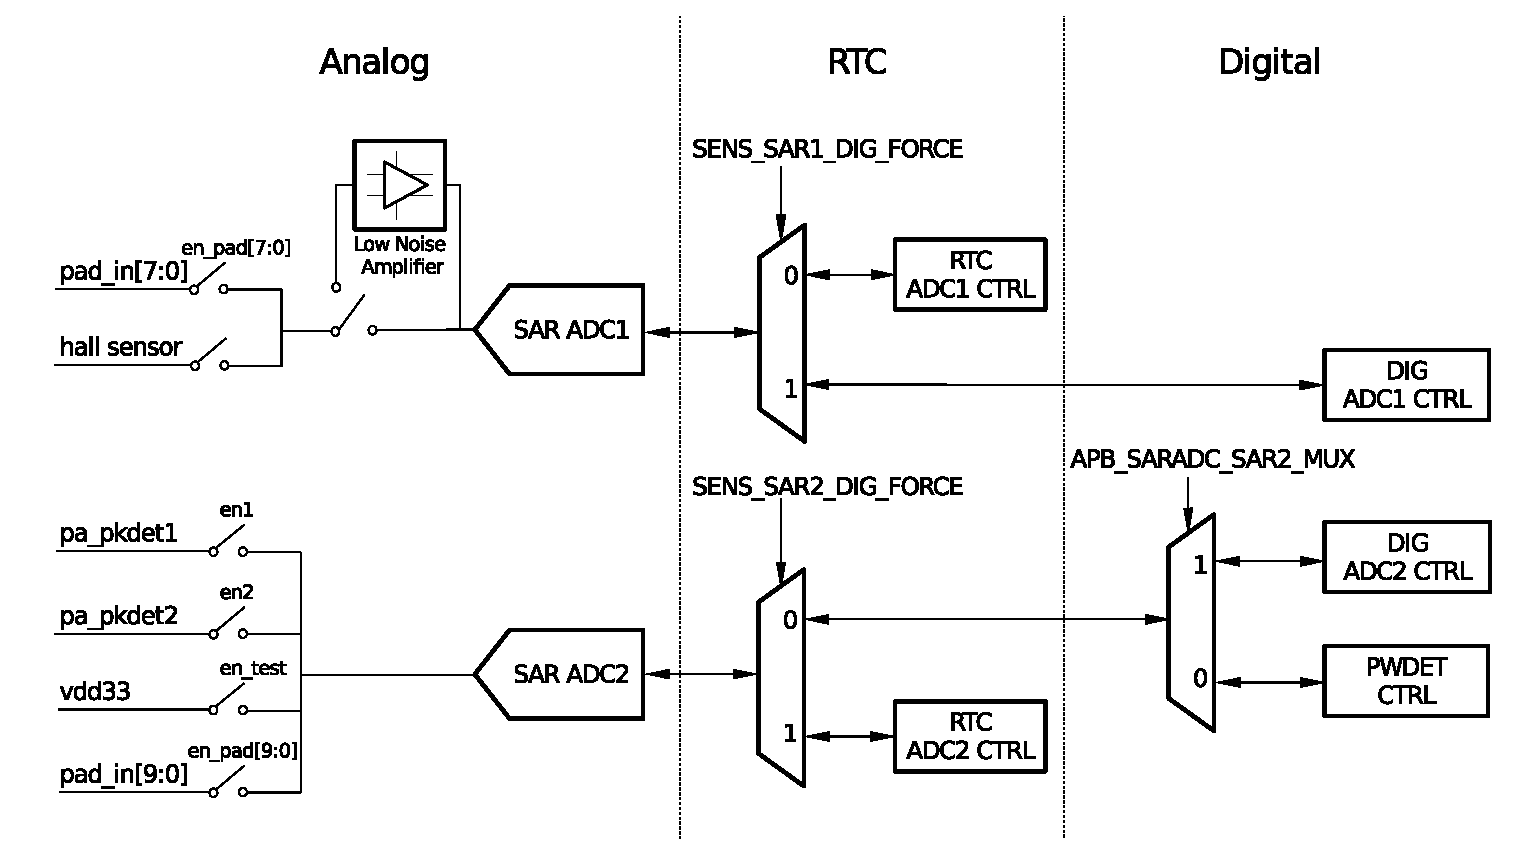
\includegraphics[width=0.9\textwidth]{./31-SENSOR/figures/saradc_mux.eps}}
    \caption{SAR ADC Outline of Function}
    \label{figure:sar adc outline of function}
\end{figure}

Table \ref{table:adc inputs} lists all the analog signals that may be sent to the SAR ADC module via the ADC channels.

\begin{longtable}{|p{5cm}|p{5cm}|p{4cm}| }
    \caption{Inputs of SAR ADC}
    \label{table:adc inputs}
    \\\hline
    \rowcolor{lightgray}
    Signal Name &  ADC Channel \# & Processed by \\\hline
    \endfirsthead
    \hline
    \rowcolor{lightgray}
    Signal Name  & ADC Channel \# & Processed by \\\hline \\\hline
    \endhead
    \hline
    \endfoot
    VDET\_2      &  7  & \multirow{8}{*}{SAR ADC1} \\ \cline{1-2}
    VDET\_1      &  6  & \\ \cline{1-2}
    32K\_XN      &  5  & \\ \cline{1-2}
    32K\_XP     &  4  & \\ \cline{1-2}
    SENSOR\_VN    &  3  & \\ \cline{1-2}
    SENSOR\_CAPN   & 2  & \\ \cline{1-2}
    SENSOR\_CAPP   &  1  & \\ \cline{1-2}
    SENSOR\_VP    &  0  & \\ \hline
    GPIO26       &  9  & \multirow{10}{*}{SAR ADC2} \\ \cline{1-2}
    GPIO25      &  8  & \\ \cline{1-2}
    GPIO27      &  7  & \\ \cline{1-2}
    MTMS         &  6  & \\ \cline{1-2}
    MTDI          &  5  & \\ \cline{1-2}
    MTCK          &  4  & \\ \cline{1-2}
    MTDO          &  3  & \\ \cline{1-2}
    GPIO2        &  2  & \\ \cline{1-2}
    GPIO0        &  1  & \\ \cline{1-2}
    GPIO4       &  0  & \\ \cline{1-2}
\end{longtable}
\vspace{-1em}
\begin{tiplisting}
\begin{itemize}
\vspace{-2em}
\item Some of the SAR ADC2 pins are used as strapping pins (GPIO0, GPIO2, and GPIO15), thus can not be used freely. 
\end{itemize}
\end{tiplisting}

There are five ADC controllers in ESP32: RTC ADC1 CTRL, RTC ADC2 CTRL, DIG ADC1 CTRL, DIG ADC2 CTRL and PWDET CTRL. The differences between them are summarized in Table \ref{table:sar adc controllers}.

\begin{longtable}[c]{|p{4.0cm}|p{2cm}|p{2cm}|p{2cm}|p{2cm}|p{2cm}|}
    \caption{ESP32 SAR ADC Controllers}
    \label{table:sar adc controllers}
    \\\hline
    \rowcolor{lightgray}
    & RTC ADC1 & RTC ADC2 & DIG ADC1 & DIG ADC2 & PWDET \\
        \hline
        \endfirsthead
        \hline
        \rowcolor{lightgray}
    & RTC ADC1 & RTC ADC2 & DIG ADC1 & DIG ADC2 & PWDET \\
        \hline
        \endhead
        \endfoot
    DAC                 & Y & - & - & - & - \\\hline
    Support deep sleep  & Y & Y & - & - & - \\\hline
    ULP coprocessor     & Y & Y & - & - & - \\\hline
    PWDET/PKDET         & - & - & - & - & Y \\\hline
    DMA                 & - & - & Y & - & - \\\hline
\end{longtable}

\subsection{RTC SAR ADC Controllers}
\label{sssec:rtcadc}

The purpose of SAR ADC controllers in the RTC power domain – RTC ADC1 CTRL and RTC ADC2 CTRL – is to provide ADC measurement with minimal power consumption in a low frequency.

The outline of a single controller's function is shown in Figure \ref{figure:sar adc ctrl}. For each controller, the start of analog-to-digital conversion can be triggered by register \hyperref[regdesc:SENSSARMEASSTART1REG]{SENS\_SAR\_MEAS\textcolor{red}{\textit{n}}\_START\_SAR}. The measurement's result can be obtained from register \hyperref[regdesc:SENSSARMEASSTART1REG]{SENS\_SAR\_MEAS\textcolor{red}{\textit{n}}\_DATA\_SAR}.

\begin{figure}[!ht]
    \centering
    \fbox{
\includegraphics[width=0.9\textwidth]{./31-SENSOR/figures/saradc_rtc_ctrl.eps}}
    \caption{RTC SAR ADC Outline of Function}
    \label{figure:sar adc ctrl}
\end{figure}

The controllers are intertwined with the ULP coprocessor, as the ULP coprocessor has a built-in instruction to start an ADC measurement. In many cases, the controllers need to cooperate with the ULP coprocessor, e.g.:
\begin{itemize}
    \item when periodically monitoring a channel during deep sleep, where the ULP coprocessor is the only trigger source during this mode;
    \item when scanning channels continuously in a sequence. Continuous scanning or DMA is not supported by the controllers. However, it is possible with the help of the ULP coprocessor.
\end{itemize}

\subsection{DIG SAR ADC Controllers}
Compared to RTC SAR ADC controllers, DIG SAR ADC controllers have optimized performance and throughput. Some of their features are:
\begin{itemize}
    \item High performance; the clock is much faster, therefore, the sample rate is highly increased.
    \item Multiple-channel scanning mode; there is a pattern table that defines the measurement rule for each SAR ADC. The scanning mode can be configured as a single mode, double mode, or alternate mode.
    \item The scanning can be started by software or I2S.
    \item DMA support; an interrupt will be generated when scanning is finished.
\end{itemize}

\begin{tiplisting}
We do not use the term “start of conversion” in this section, because there is no direct access to starting a single SAR analog-to-digital conversion. We use “start of scan” instead, which implies that we expect to scan a sequence of channels with DIG ADC controllers.
\end{tiplisting}

Figure \ref{figure:dig adc overview} shows a diagram of DIG SAR ADC controllers.

\begin{figure}[H]
    \centering
    
\includegraphics[width=0.8\textwidth]{./31-SENSOR/figures/saradc_dma}
    \caption{Diagram of DIG SAR ADC Controllers}
    \label{figure:dig adc overview}
\end{figure}

The pattern tables contain the measurement rules mentioned above. Each table has 16 items which store information on channel selection, resolution and attenuation. When scanning starts, the controller reads measurement rules one-by-one from a pattern table. For each controller the scanning sequence includes 16 different rules at most, before repeating itself.

The 8-bit item (the pattern table register) is composed of three fields that contain channel, resolution and attenuation information, as shown in Table \ref{table:pattern table register}.

\begin{table}[H]
    \caption{Fields of the Pattern Table Register}
    \label{table:pattern table register}
    \centering
    \begin{tabular}[c]{|p{5cm}|p{5cm}|p{5cm}|}
        \hline
        \rowcolor{lightgray}
        \multicolumn{3}{|c|}{Pattern Table Register [7:0]} \\
        \hline
        ch\_sel[3:0] & bit\_width[1:0] & atten[1:0] \\
        \hline
        channel to be scanned & resolution & attenuation \\
        \hline
    \end{tabular}
\end{table}

There are three scanning modes: single mode, double mode and alternate mode.

\begin{itemize}
    \item Single mode: channels of either SAR ADC1 or SAR ADC2 will be scanned.
    \item Double mode: channels of SAR ADC1 and SAR ADC2 will be scanned simultaneously.
    \item Alternate mode: channels of SAR ADC1 and SAR ADC2 will be scanned alternately.
\end{itemize}

ESP32 supports up to a 12-bit SAR ADC resolution. The 16-bit data in DMA is composed of the ADC result and some necessary information related to the scanning mode:

\begin{itemize}
    \item For single mode, only 4-bit information on channel selection is added.
    \item For double mode or alternate mode, 4-bit information on channel selection is added plus one extra bit indicating which SAR ADC was selected.
\end{itemize}

For each scanning mode there is a corresponding data format, called Type \uppercase\expandafter{\romannumeral1} and Type \uppercase\expandafter{\romannumeral2}. Both data formats are described in Tables \ref{table:type i dma data format} and \ref{table:type ii dma data format}.

\begin{table}[H]
    \caption{Fields of Type \uppercase\expandafter{\romannumeral1} DMA Data Format}
    \label{table:type i dma data format}
    \centering
    \begin{tabular}[c]{|p{7.75cm}|p{7.75cm}|}
        \hline
        \rowcolor{lightgray}
        \multicolumn{2}{|c|}{\textbf{Type I} DMA Data Format [15:0]} \\
        \hline
        ch\_sel[3:0] & data[11:0] \\
        \hline
        channel & SAR ADC data \\
        \hline
    \end{tabular}
\end{table}

\begin{table}[H]
    \caption{Fields of Type \uppercase\expandafter{\romannumeral2} DMA Data Format}
    \label{table:type ii dma data format}
    \centering
    \begin{tabular}[c]{|p{5cm}|p{5cm}|p{5cm}|}
        \hline
        \rowcolor{lightgray}
        \multicolumn{3}{|c|}{\textbf{Type \uppercase\expandafter{\romannumeral2}} DMA Data Format [15:0]} \\
        \hline
        sar\_sel & ch\_sel[3:0] & SAR ADC data[10:0] \\
        \hline
        SAR ADCn & channel & SAR ADC data \\
        \hline
    \end{tabular}
\end{table}

For Type \uppercase\expandafter{\romannumeral1} the resolution of SAR ADC is up to 12 bits, while for Type \uppercase\expandafter{\romannumeral2} the resolution is 11 bits at most.

DIG SAR ADC Controllers allow the use of I2S for direct memory access. The WS signal of I2S acts as a measurement-trigger signal. The DATA signal provides the information that the measurement result is ready. Software can configure \hyperref[regdesc:APBSARADCCTRLREG]{APB\_SARADC\_DATA\_TO\_I2S}, in order to connect ADC to I2S.

\section{DAC}
\label{ssec:dac}

\subsection{Introduction}

Two 8-bit DAC channels can be used to convert digital values into analog output signals (up to two of them). The design structure is composed of integrated resistor strings and a buffer. This dual DAC supports power supply and uses it as input voltage reference. The dual DAC also supports independent or simultaneous signal conversions inside of its channels.

\subsection{Features}

The features of DAC are as follows:
\begin{itemize}
    \item Two 8-bit DAC channels
    \item Independent or simultaneous conversion in channels
    \item Voltage reference from the VDD3P3\_RTC pin
    \item Cosine waveform (CW) generator
    \item DMA capability
    \item Start of conversion can be triggered by software or SAR ADC FSM (please refer to the \hyperref[ssec:saradc]{SAR ADC chapter} for more details)
    \item Can be fully controlled by the ULP coprocessor
\end{itemize}

A diagram showing the DAC channel's function is presented in Figure \ref{figure:dac mux}. For a detailed description, see the sections below.

\begin{figure}[!ht]
    \centering
    \fbox{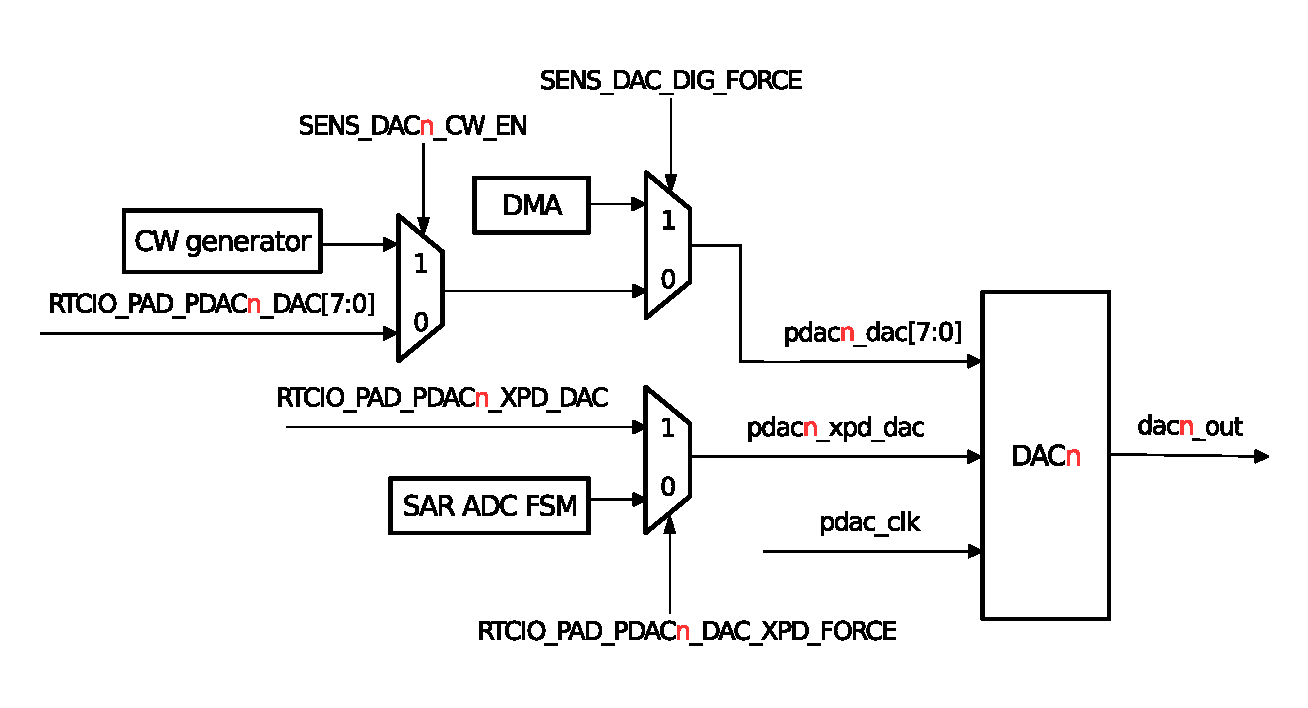
\includegraphics[width=0.7\textwidth]{./31-SENSOR/figures/dac.eps}}
    \caption{Diagram of DAC Function}
    \label{figure:dac mux}
\end{figure}

\subsection{Structure}\label{sec:structure}

The two 8-bit DAC channels can be configured independently. For each DAC channel, the output analog voltage can be calculated as follows:
$$\mathrm{DAC\textcolor{red}{\textit{n}}\_OUT = VDD3P3\_RTC \cdot PDAC\textcolor{red}{\textit{n}}\_DAC / 255}$$ 

\begin{itemize}
    \item VDD3P3\_RTC is the voltage on pin VDD3P3\_RTC (typically 3.3V).
    \item PDAC\textcolor{red}{\it{n}}\_DAC has multiple sources: \hyperref[ssec:cosine gen]{CW generator}, register \hyperref[regdesc:RTCIOPADDAC1REG]{RTCIO\_PAD\_DAC\textcolor{red}{\it{n}}\_REG}, and DMA.
\end{itemize}

The start of conversion is determined by register \hyperref[regdesc:RTCIOPADDAC1REG]{RTCIO\_PAD\_PDAC\textcolor{red}{\textit{n}}\_XPD\_DAC}. The conversion process itself is controlled by software or SAR ADC FSM; see Figure \ref{figure:dac mux}.

\subsection{Cosine Waveform Generator}
\label{ssec:cosine gen}

The cosine waveform (CW) generator can be used to generate a cosine / sine tone. A diagram showing cosine waveform generator’s function is presented in Figure \ref{figure:cw gen}.

The CW generator has the following features:
\begin{itemize}
    \item Adjustable frequency\\
    The frequency of CW can be adjusted by register \hyperref[regdesc:SENSSARDACCTRL1REG]{SENS\_SAR\_SW\_FSTEP[15:0]}:
    $$\mathrm{freq = dig\_clk\_rtc\_freq \cdot SENS\_SAR\_SW\_FSTEP / 65536}$$
    The frequency of dig\_clk\_rtc is typically 8 MHz.
    \item Scaling\\
    Configuring register \hyperref[regdesc:SENSSARDACCTRL2REG]{SENS\_SAR\_DAC\_SCALE\textcolor{red}{\textit{n}}[1:0]}; the amplitude of a CW can be multiplied by 1, 1/2, 1/4 or 1/8.
    \item DC offset\\
    The offset may be introduced by register \hyperref[regdesc:SENSSARREADCTRL2REG]{SENS\_SAR\_DAC\_DC\textcolor{red}{\textit{n}}[7:0]}. The result will be saturated.
    \item Phase shift\\
    A phase-shift of 0 / 90 / 180 / 270 degrees can be added by setting register \hyperref[regdesc:SENSSARDACCTRL2REG]{SENS\_SAR\_DAC\_INV\textcolor{red}{\textit{n}}[1:0]}.
\end{itemize}

\begin{figure}[!ht]
    \centering
    \fbox{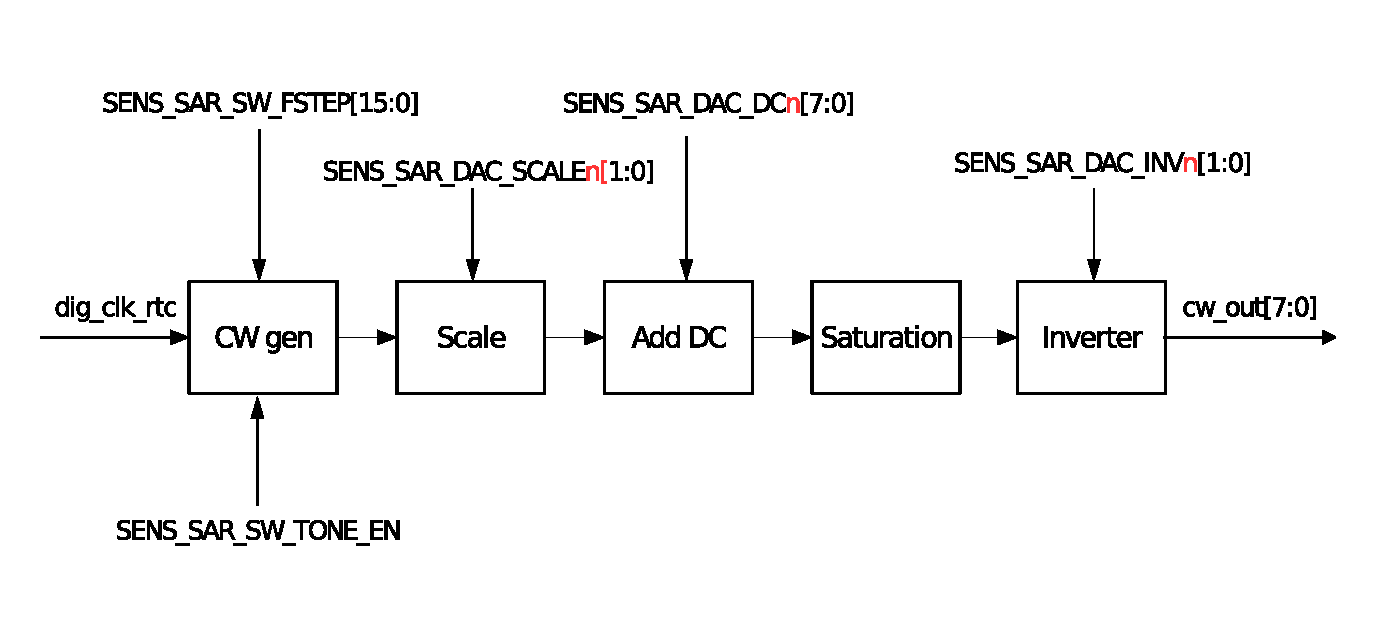
\includegraphics[width=0.7\textwidth]{./31-SENSOR/figures/dac2.eps}}
    \caption{Cosine Waveform (CW) Generator}
    \label{figure:cw gen}
\end{figure}

\subsection{DMA support}

A DMA controller with dual DMA channels can be used to set the output of two DAC channels.
By configuring \hyperref[regdesc:SENSSARDACCTRL1REG]{SENS\_SAR\_DAC\_DIG\_FORCE}, I2S\_clk can be connected to DAC clk, and I2S\_DATA\_OUT can be connected to DAC\_DATA for direct memory access.

For details, please refer to chapter \hyperref[paragraph: DMA]{DMA}.
\vspace{-1em}

\hypertarget{sensor-reg-summ}{}
\section{Register Summary}

Note: The registers listed below have been grouped, according to their functionality. This particular grouping does not reflect the exact sequential order of their place in memory.

The abbreviations given in Column \textbf{Access} are explained in Section \hyperref[glossary-access-types]{\textit{Access Types for Registers}}.


\subsection{Sensors}\label{sec:sensor-reg-summ}

\subfile{\modulefiles/On_Chip_Sensor_sens_reg_summary_en.tex}

\subsection{Advanced Peripheral Bus}\label{sec:apb-reg-summ}

The abbreviations given in Column \textbf{Access} are explained in Section \hyperref[glossary-access-types]{\textit{Access Types for Registers}}.

\subfile{\modulefiles/On_Chip_Sensor_apb_ctrl_reg_summary_en.tex}

\subsection{RTC I/O}

For details, please refer to Section \hyperref[section:4.12]{Register Summary} in Chapter \hyperref[mod:iomuxgpio]{IO\_MUX and GPIO Matrix}.


\newpage
\section{Registers}
\label{section:registers}

\subsection{Sensors}

The addresses in this section are relative to (the RTC base address + 0x0800) provided in Table \ref{table:Peripheral_Address_Mapping} in Chapter \ref{mod:sysmem} \textit{\nameref{mod:sysmem}}. The absolute register addresses are listed in Section \ref{sec:sensor-reg-summ} \textit{\nameref{sec:sensor-reg-summ}}. 

For how to program reserved fields, please refer to Section \hyperref[programming-reserved-field]{\textit{Programming Reserved Register Field}}.

\subfile{\modulefiles/On_Chip_Sensor_sens_reg_en.tex}

\subsection{Advanced Peripheral Bus}

The addresses in this section are relative to the base address of 0x6000\_2600 (by AHB bus). The absolute register addresses are listed in Section \ref{sec:apb-reg-summ} \textit{\nameref{sec:apb-reg-summ}}.

For how to program reserved fields, please refer to Section \hyperref[programming-reserved-field]{\textit{Programming Reserved Register Field}}.

\subfile{\modulefiles/On_Chip_Sensor_apb_ctrl_reg_en.tex}

\subsection{RTC I/O}

For details, please refer to Section \hyperref[section:4.12]{Registers} in Chapter \hyperref[mod:iomuxgpio]{IO\_MUX and GPIO Matrix}.

\end{document}
